%
% Documento: Introdu\c{c}\~{a}o
%

\chapter{INTRODU\c{c}\~{a}O}\label{chap:introducao}

O cenário atual dos negócios objetiva a diferenciação e a busca por um desempenho com base na eficiência, seja em uma organiza\c{c}\~{a}o pública ou privada, dar-se-\'{a} por meio da utilização de ferramentas e recursos, que visam a otimiza\c{c}\~{a}o das atividades, paralelamente à redução de seus custos.

Assim, na \'{a}rea da seguran\c{c}a pública e por intermédio dos elementos da tecnologia de informação, é possível registrar, armazenar e ter acesso de maneira eficaz, organizada e estruturada as informações sobre uma grande massa de dados de denúncias e ocorrências em cidades, bairros com datas e horas. Desta forma, tendências podem ser analisadas com base nesses dados, viabilizando a aplica\c{c}\~{a}o de determinado tipo de policiamento e ajudando na gestão da própria seguran\c{c}a pública, além de permitir uma melhor interlocução dos participantes da SSP.

\section{Apresenta\c{c}\~{a}o}

Na \'{a}rea da seguran\c{c}a pública e por intermédio dos elementos da tecnologia de informação, é possível registrar, armazenar e ter acesso de maneira eficaz, organizada e estruturada as informações sobre uma grande massa de dados de denúncias e ocorrências em cidades, bairros com datas e horas. Desta forma, tendências podem ser analisadas com base nesses dados, viabilizando a aplica\c{c}\~{a}o de determinado tipo de policiamento e ajudando na gestão da própria seguran\c{c}a pública, além de permitir uma melhor interlocução dos participantes da SSP.

Neste trabalho aplicamos as t\'{e}cnicas de Kimbal (2013)\cite{dw-kimball-2013} apresentadas em sua obra \textit{The Data Warehouse Toolkit}, no desenvolvimento de um BI que atue no banco de dados que registra as informa\c{c}ões das denúncias para ampliar a habilidade de planejar e auxiliar \`{a} tomada de decisões estrat\'{e}gicas no âmbito da Secretaria de Seguran\c{c}a Pública do Estado de Alagoas. 

Neste trabalho, propõe-se aplicar essa t\'{e}cnica com o uso de ferramentas modernas tal como o Pentaho \index{NewR}\footnote{Pentaho: Plataforma ou Software da Empresa Hitachi, composta por v\'{a}rias ferramentas que empregam as t\'{e}cnicas de BI.} na base de dados de denúncias registradas. Utilizaremos uma amostra de dados que abrangem os três primeiros meses do ano de 2020, os mesmo foram pesquisados e salvos no formato do \textit{Microsoft Excel}, que passaram pelo processo de extra\c{c}\~{a}o, transforma\c{c}\~{a}o e leitura e ao final termos um conjunto complexo de informa\c{c}ões que ajudar\~{a}o na tomada de decis\~{a}o.

% Disque Denúncia
\section{História do Disque Denúncia}		

Desde sua implanta\c{c}\~{a}o em Alagoas, em outubro de 2011, o Disque-Denúncia tem se revelado uma ferramenta útil para a popula\c{c}\~{a}o, que passou a contar com um meio seguro e sigiloso para relatar denúncias diversas.
Atrav\'{e}s do número telefônico 181, \'{e} possível denunciar ocorrências de criminalidade com a garantia do sigilo de quem passa a informa\c{c}\~{a}o. Al\'{e}m disso, o servi\c{c}o atua em denúncias referentes \`{a} venda ilegal de g\'{a}s de cozinha, tr\'{a}fico de drogas, posse e porte ilegal de arma de fogo, localiza\c{c}\~{a}o de foragidos e pessoas envolvidas com roubo a banco e pr\'{a}tica de homicídio.

Ele \'{e} gerido pela Secretaria de Seguran\c{c}a Pública, o número 181 \'{e} uma central de atendimento a recep\c{c}\~{a}o de chamadas telefônicas com denúncias de crimes e delitos que tem como objetivo agilizar o atendimento \`{a} popula\c{c}\~{a}o e contribuir para a redu\c{c}\~{a}o da criminalidade no Estado. \'{e} um servi\c{c}o gratuito e totalmente sigiloso. Por isso, o anonimato, al\'{e}m de um direito, se torna um dever da central desse servi\c{c}o, para garantir a seguran\c{c}a do cidad\~{a}o denunciante.

O anonimato \'{e} garantido porque, as liga\c{c}ões para o Disque Denúncia n\~{a}o s\~{a}o identificadas, rastreadas ou gravadas. Ao ligar para o 181, o usu\'{a}rio receber\'{a} uma senha num\'{e}rica chamada código da denúncia. Esta ser\'{a} a referência dele em caso do mesmo precisar acompanhar o andamento da investiga\c{c}\~{a}o, ou trazer novas informa\c{c}ões sobre o caso.

No SisGOU, os dados aparecem no módulo Disque Denúncia, eles s\~{a}o vindos do site do disque denúncia ser\'{a} apresentado nas próximas se\c{c}ões. Esses dados das denúncias,  guardando o sigilo e identifica\c{c}\~{a}o de quem entra em contato com o servi\c{c}o, que pode ser atrav\'{e}s do ``APP 181'', disponível na \textint{Play Store} \index{NewR}\footnote{Play Store: \'{e} uma loja virtual que j\'{a} vem pr\'{e}-instalada em aparelhos certificados, permitindo o acesso ao conteúdo digital, incluindo aplicativos, jogos, filmes, músicas e livros.} e no portal do servi\c{c}o, conforme figura abaixo, assim pode-se realizar denúncias via celular ou \textit{tablet}, pela internet ou liga\c{c}\~{a}o para o número 181, esse último sendo o mais conhecido, auxiliando no controle das denúncias e no envio das mesmas para as Unidades e Companhias de Polícia Militar e para as Delegacias, por\'{e}m n\~{a}o possui nenhuma ferramenta de inteligência de negócios integrada ao sistema, que venha orientar os gestores na tomada de decisões. 

### Figuras
\begin{figure}[H]
	\vspace*{0,2cm}
    \centering
    \caption{Disque Denúncia \textit{Mobile}}
    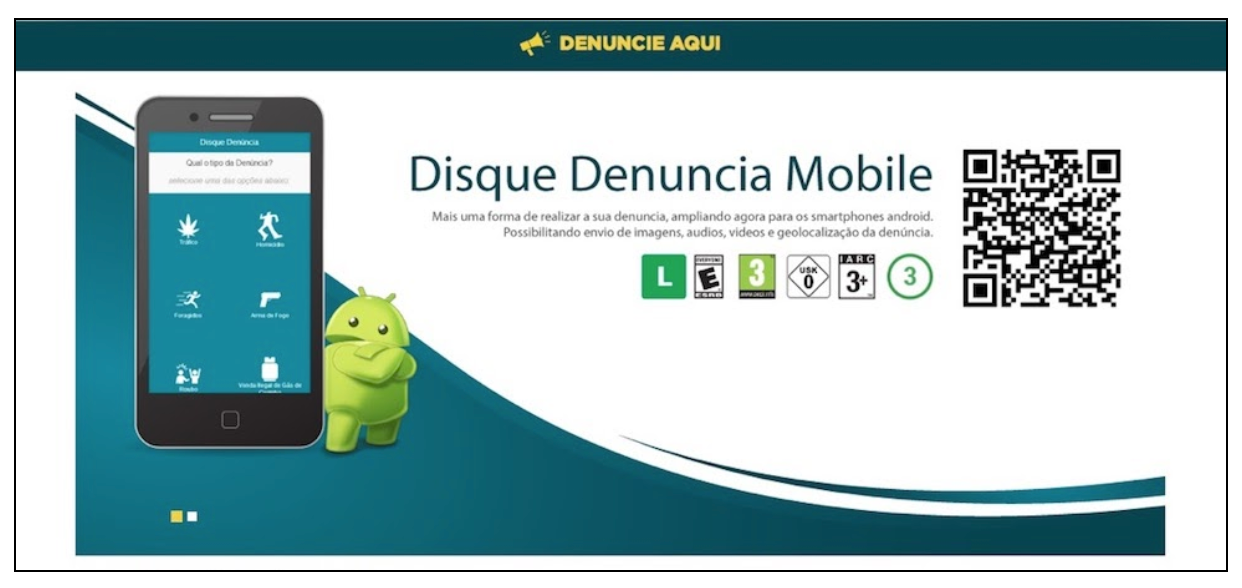
\includegraphics[width=0.6\textwidth]{./04-figuras/figura-disque-denuncia}
    \label{fig:ilustfigdisquedenuncia}
\end{figure}
\vspace*{-0,9cm}
{\raggedright \fonte{Autor desta monografia, 2020.}} \\

A partir dos dados do Disque-Denúncia, com base nos últimos seis anos, 63\% das liga\c{c}ões se referem a fatos em Maceió. Desde a implanta\c{c}\~{a}o desse servi\c{c}o, que funciona 24 horas, registra-se aumento anual no número de denúncias. At\'{e} 2011, havia uma m\'{e}dia de sete ao dia. Em 2016 este dado subiu para 42 (quarenta e dois) registros di\'{a}rios, sendo um acr\'{e}scimo de 5\% em rela\c{c}\~{a}o a 2017 nas informa\c{c}ões passadas pela popula\c{c}\~{a}o, hoje se tornando uma ferramenta importante para a SSP/AL.

% Objetivo Geral
\subsection{Objetivo geral}

O objetivo deste trabalho é desenvolver e implantar um modelo de \textint{Data Warehouse} Corporativo com base nos dados provindos do Aplicativo SISGOU da SSP/AL que cont\'{e}m os dados do 181, aplicando t\'{e}cnicas de DW/BI, Segundo KIMBALL (2013)\cite{dw-kimball-2013}.

% Objetivo Específico
\subsection{Objetivos específicos}

Os objetivos específicos do presente trabalho de pesquisa s\~{a}o:

\begin{itemize}

    \item Revisar as literaturas que abrangem os principais conceitos de BI; 
    \item Identificar problemas e benefícios com relação à implementação da tecnologia  \textint{e data warehouse};
    \item Definir um repositório de dados históricos para auxiliar os gerentes, contendo informações relevantes para a tomada de decisões com base nos dados armazenados;
    \item Extrair informações da base de dados do SISGOU, integrá-las e armazená-las em um repositório único central de \textint{Data Warehouse};
    \item Definir os níveis de granularidades necessários para a distribuição dos dados dentro deste modelo dimensional distribuído;
    \item Repassar à sociedade os conhecimentos e resultados obtidos nesta pesquisa.

\end{itemize}

% Resultados esperados
\section{Resultados Esperados}

Os resultados esperados s\~{a}o:

\begin{itemize}

    \item Após aplicarmos as t\'{e}cnicas de KIMBALL (2013) termos um DW funcional;
    \item Explorar o DW criado com as t\'{e}cnicas acima para prover informa\c{c}ões gerenciais;
    \item Aplicar estas informa\c{c}ões gerenciais para melhorar o Policiamento Ostensivo;
    \item Prover pain\'{e}is \textint{(Dashboards)} eficientes e que ajudem com informa\c{c}ões que auxiliem nas tomadas de decisões
    \item Tornar esse trabalho como base para o uso de recursos de BI para ajudar na seguran\c{c}a pública.

\end{itemize}